\documentclass[conference]{IEEEtran}
\usepackage{graphicx}
\usepackage{lmodern}


% path gambar
\graphicspath{{./picture/}}

% JUDUL %%%%%%%%%%%%%%%%%%%%%%%%%%%%%%%%%%%%%%%%%%%%%%%%%%%%%
\title{Mengirim Data Signal Strength Hasil Pemindaian Jaringan WiFi ke Telegram Bot dengan NodeMCU ESP32}

% PENULIS %%%%%%%%%%%%%%%%%%%%%%%%%%%%%%%%%%%%%%%%%%%%%%%%%%%
\author{Arvy Kurnia Ramadhan\IEEEauthorrefmark{1},Bimo Aryo Pratama\IEEEauthorrefmark{2},Armando Mendoza Putra\IEEEauthorrefmark{3}, Fajri Rahmat Ilahi\IEEEauthorrefmark{4}\\
\textit{Fakultas Teknologi Informasi}\\
\textit{Teknik Komputer}\\
\textit{Institut Teknologi Batam}\\
Batam, Indonesia\\
Email: \{\IEEEauthorrefmark{1}2022009,\IEEEauthorrefmark{2}2022008,\IEEEauthorrefmark{3}2022012,\IEEEauthorrefmark{4}2022013\}@student.iteba.ac.id}

\begin{document}
% untuk mengeluarkan judul dan author
\maketitle
% ABSTRAK %%%%%%%%%%%%%%%%%%%%%%%%%%%%%%%%%%%%%%%%%%%%%%%%%%
\begin{abstract}
    Dalam sistem komunikasi data nirkabel, penggunaan WiFi menjadi pilihan banyak pengguna karena mobilitas dan kecepatan transfer datanya. Kualitas kekuatan sinyal berperan besar dalam layanan komunikasi data ini, sehingga penting untuk mengetahui kualitas kekuatan sinyal pada jaringan WiFi. Pemindaian jaringan WiFi menggunakan perangkat NodeMCU V3 dapat mengukur kekuatan sinyal masing-masing jaringan, kemudian data hasil pemindaian dan pengukuran kekuatan sinyal dikirimkan ke Telegram menggunakan channel BotFather melalui web server agar dapat diketahui hasilnya.
\end{abstract}
\vspace{0.2cm}
% kata kunci %%%%%%%%%%%%%%%%%%%%%%%%%%%%%%%%%%%%%%%%%%%%%%%%
\begin{IEEEkeywords}
    \emph{WiFi}, \emph{signal strength}, \emph{NodeMCU V3}, \emph{TelegramBot}, \emph{BotFather}
\end{IEEEkeywords}
% pendahuluan %%%%%%%%%%%%%%%%%%%%%%%%%%%%%%%%%%%%%%%%%%%%%%
\section{Pendahuluan}
Perkembangan teknologi merupakan hal yang sejalan dengan 
perkembangan zaman, dimana masyarakat kini selalu
menginginkan berbagai hal agar dapat dilakukan secara otomatis
ataupun dari jarak jauh. Perkembangan smarthome dengan
kontrol jarak jauh menjadi salah satu fokus utama dalam
perkembangan teknologi dimana pengontrolannya dilakukan dari
jarak jauh dan secara real time dan diharapkan pula bagi generasi
masa kini untuk dapat mengimplementasikan beberapa bagian
dari teknologi yang cukup sederhana dalam lingkungan masyarakat. ada
beberapa teknik analisis yang di gunakan untuk menentukan
sistem, perangkat dan juga bagaimana pengaplikasiannya. Maka
dari itu dipilihlah Telegram bot sebagai interface antara perangkat
dan pengguna dimana board ESP32 Module sebagai pusat
kontrolnya dan pemrogramannya menggunakan Ardiono IDE.
Semua hal ini masih perlu di pelajari terlebih dahulu dengan
dukungan berbagai jurnal penelitian ,
    
    Setelah proses analisis dilakukan maka akan didapat hasil
berupa suatu sistem notifikasi scanner yang di program untuk dapat
dikontrol dari jarak jauh. Pengontrolan ini dilakukan dengan
bantuan internet sebagai media penghubungnya dan juga Bot
Telegram sebagai media penginputan perintah yang diberikan
dengan jarak yang jauh apabila terdapat koneksi internet 
antara perangkat penerima dan juga pengirim.


\section{Penjelasan}
\subsection{Bot Telegram}
\vspace{0.2cm}
\begin{figure}[h]
    \centering
    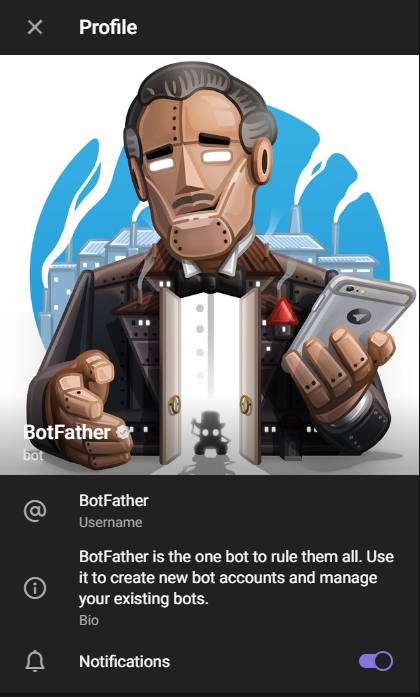
\includegraphics[width=0.2\textwidth]{Botfather.png}
    \caption{BotFather Telegram}
\end{figure}

    Telegram adalah salah satu aplikasi layanan pengirim pesan instan multiplatform. Bot Telegram 
    sendiri merupakan salah satu fitur dari Telegram yang mana funginya untuk
    mempermudah kegiatan dalam mengakses Telegram. Bot itu sendiri
    berasal dari kata robot atau mesin pekerja yang meringkankan pekerjaan.
    Bot di dalam telegram bekerja dengan cara inputan perintah yang buat.
    Dalam pengaturan atau pebuatan bot telegram ada dua cara yang 
    bisa dilakukan, yang pertama dengan membuat program dengan bahasa
    mesin lalu diinput ke protokol telegram. dan yang kedua yaitu dengan
    meminta akses bot telegram ke BotFather.
   
    
        Membuat bot Telegram dengan meminta Akses kepada BotFather dilakukan untuk
    mendapatkan kode API, kode ini merupakan kode unik khusus bagi suatu
    akun Bot Telegram untuk Koneksi dengan sistem di luar Telegram itu
    sendiri. Cara kerja kode ini mirip seperti nomor HP, yang mana setiap
    penguna Bot Telegram memiliki kode API tersendiri dan tidak dapat di copy
    oleh orang lain, namun jika pengguna ingin mengubah kode API yang
    dimilikinya bisa dilakukan dengan cara menghapus Bot Telegram lalu
    membuat ulang Bot Telegram dengan IDE yang sama.
    BotFather sendiri merupakan suatu Fitur AI milik Telegram yang
    mengatur pembuatan Bot Telegram yang bekerja otomatis, sistem
    BotFather ini lebih merujuk ke sistem pembalasan pesan otomatis yang
    mana pemeberian kode API yang diberikan dilakukan secara acak.


    \subsection{NodeMCU}
    NodeMCU ESP32 adalah serangkaian sistem berbiaya rendah dan berdaya rendah pada mikrokontroler chip dengan Wi-Fi terintegrasi dan Bluetooth mode ganda. Seri chip ESP32 meliputi ESP32-D0WDQ6, ESP32-D0WD, ESP32-D2WD, dan ESP32-S0WD. Mikrokontroler ini cocok untuk berbagai aplikasi, termasuk otomatisasi rumah, perangkat IoT (Internet of Things), dan perangkat elektronik yang dapat dikenakan. Seri mikrokontroler ESP32 didasarkan pada mikroprosesor ESP32, yang merupakan mikroprosesor berdaya rendah dengan prosesor dual-core dan Wi-Fi on-chip dan radio Bluetooth.

    NodeMCU versi 0.9 diluncurkan pada 13 Oktober 2014 oleh user bernama Hong pada GitHub setahun setelah diproduksinya ESP32 pada 30 Desember 2013. ESP32 merupakan SoC yang memiliki module wifi sebagai perangkat tambahan mikrokontroller agar dapat terhubung dengan wifi dan membuat koneksi TCP/IP.

    NodeMCU merupakan sebuah platform IoT yang bersifat open source dan juga include dengan module ESP 12, dan berjalan pada firmware esp32 yang menjadikan NodeMCU sebuah mikrokontroller yang telah dilengkapi dengan module Wifi didalamnya.

    \begin{figure}[h]
        \centering
        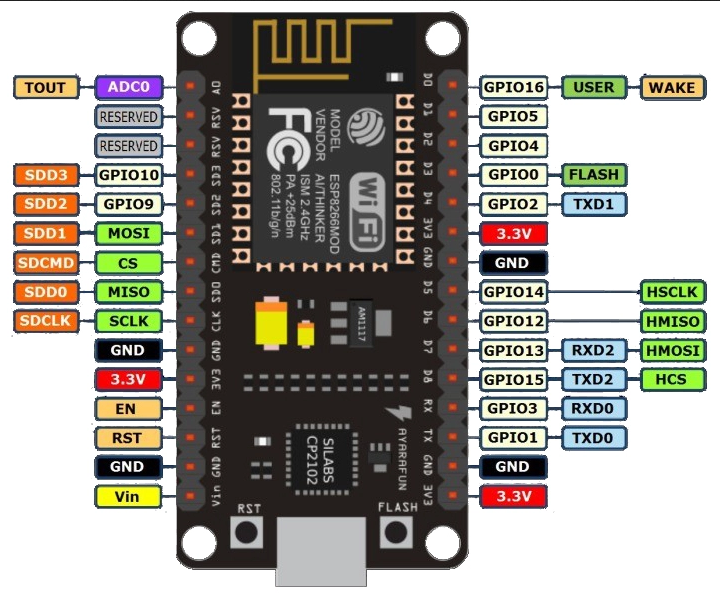
\includegraphics[width=0.3\textwidth]{Nodem.png}
        \caption{GPIO NodeMCU V2}
    \end{figure}

    NodeMCU berfungsi sama seperti Arduino, walaupun dengan IC, GPIO, dan Bahasa program yang digunakan berbeda tetapi tujuannya sama yaitu untuk mengontrol suatu system, dan kelebihannya dibandingkan arduino yaitu telah include dengan module Wifi yang tertanam pada systemnya.

    
    
\section{Hasil dan Pembahasan}
\subsection{Flowcart Telegram Bot}
\begin{figure}[h]
    \centering
    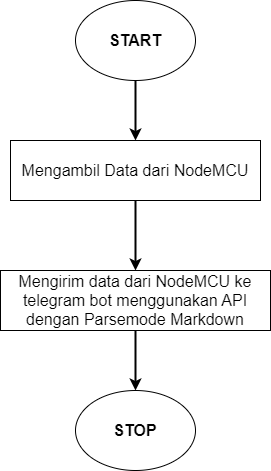
\includegraphics[width=0.2\textwidth]{Flowchart telegram bot.png}
    \caption{Flowchart Telegram Bot}
\end{figure}
\vspace{0cm}

\subsection{Flowchart NodeMCU}
\begin{figure}[h]
    \centering
    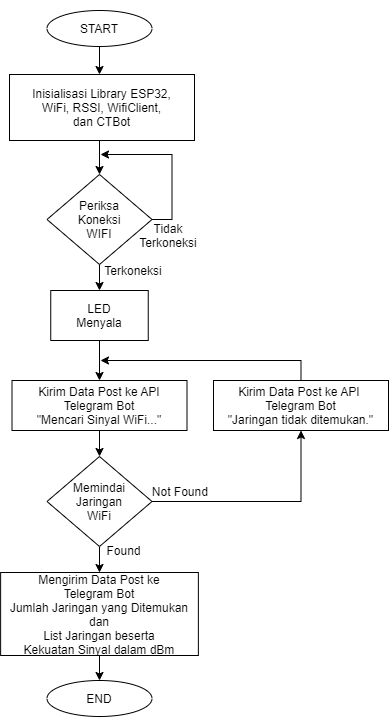
\includegraphics[width=0.2\textwidth]{Flowchart NodeMCU telegram bot.png}
    \caption{Flowchart NodeMCU}
\end{figure}
\vspace{0cm}
\subsection{Cara Kerja Program}
Berikut adalah langkah untuk membuat program. Masukan token bot atau API, kemudian inisialisasi library CTBot.h. Buat function untuk mengirim data NodeMCU ke API Telegram Bot.

Cara penggunaan Telegram Bot Kelompok 8 klik tombol /start atau ketik /start pada telegram bot. Setelah itu bot akan mengirimkan pesan untuk list command yang bisa digunakan di dalam bot.
Gunakan command /scan untuk memulai scanning mengukur kekuatan jaringan sinyal WiFi.
Setelah itu NodeMCU akan memulai scanning dan membaca data yang kemudian akan dikirimkan ke API telegram bot.
\subsection{Data Hasil Pengukuran}
\subsubsection{Hasil Pengukuran Didalam Rumah}
Berikut ini perhitungan menggunakan persamaan RSSI 
pada jaringan wireless yang ada disekitar rumah terhadap pengahalang

    \begin{table}[htbp]
    \caption{Table Analisis Pengukuran RSSI}
    \begin{center}
    \begin{tabular}{|c|c|c|}
        \hline
    \textbf{SSID}&\textbf{\textit{RSSI}}& \textbf{\textit{Penerima Sinyal}} \\
    \hline
    realme 6 & -51 dBm & 98  \\
    \hline
    PUPUT & -65 dBm & 70  \\
    \hline
    BOL & -87 dBm & 26   \\
    \hline
    Office & -87 dBm & 26  \\
    \hline
    OPPO A15S & -88 dBm & 24  \\
    \hline
    Double D 3a & -91 dBm & 18  \\
    \hline
    Double D 4a & -91 dBm & 18  \\
    \hline
    Double D 5a & -92 dBm & 16  \\
    \hline
    \multicolumn{3}{l}{$^{\mathrm{1}}$Hasil scanning Nodemcu Ke Telegram Bot}
    \end{tabular}
    \label{tab1}
    \end{center}
    \end{table}

    \subsubsection{Hasil Pengukuran Diluar rumah}
    Berikut ini perhitungan menggunakan persamaan RSSI 
pada jaringan wireless yang ada diluar rumah
 terhadap pengahalang seperti pepohonan dan intervensi objek lain nya dengan studi kasus dimana dalam 1 access
 point dibagi menjadi beberapa SSID pada tabel berikut ini : 

 \begin{table}[htbp]
    \caption{Table Analisis Pengukuran RSSI}
    \begin{center}
    \begin{tabular}{|c|c|c|}
        \hline
    \textbf{SSID} &  \textbf{\textit{Penerimaan Sinyal}}& \textbf{\textit{RSSI}} \\
    \hline
    realme 6 & 100 & -39 dBm   \\
    \hline
    PUPUT & 52 & -74 dBm   \\
    \hline
    The Li Internet & 38 & -81 dBm   \\
    \hline
    Li Guest  & 36 & -82 dBm   \\
    \hline
    OPPO A15S  & 26 & -87 dBm   \\
    \hline
    Biz D82  & 20 & -90 dBm   \\
    \hline
    Nisilco  & 18 & -91 dBm   \\
    \hline
    biduan  & 18 & -91 dBm   \\
    \hline
    Jesslyn Brayden  & 16 & -92 dBm   \\
    \hline
    Double D 3a  & 8 & -96 dBm   \\
    \hline

    \multicolumn{3}{l}{$^{\mathrm{2}}$Hasil scanning Nodemcu Ke Telegram Bot}
    \end{tabular}
    \label{tab2}
    \end{center}
    \end{table}


    \subsection{Percobaan Telegram Bot}
    Berikut ini adalah hasil percobaan menggunakan telegram bot.
    \begin{figure}[h]
        \centering
        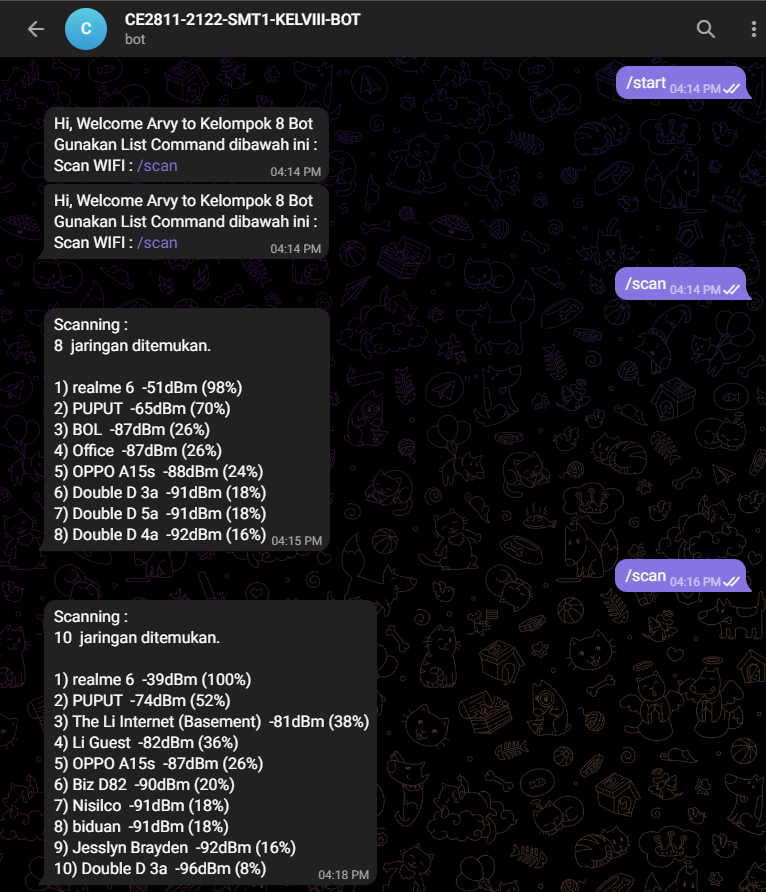
\includegraphics[width=0.4\textwidth]{telebott.png}
    \end{figure}

    

\subsection{Pengaruh Besar nya Kekuatan sinyal}



Kekuatan sinyal RSSI yang diterima penerima tidak hanya bergantung pada jarak antara pemancar dan penerima, tetapi juga menunjukkan variasi yang signifikan akibat fading dan shadowing pada lokasi tertentu. Hal ini terlihat pada tempat-tempat penelitian dimana lingkungan sekitar memiliki banyak sifat seperti dinding, lemari, meja dan sifat-sifat lainnya di dalam ruangan, yang dapat menyebabkan pelemahan sinyal, defleksi sinyal, dan pantulan sinyal, sehingga terjadi penurunan kekuatan sinyal. dipancarkan oleh pemancar ke penerima, meskipun jarak antara pemancar dan penerima dekat, tetapi terhalang oleh properti sekitarnya, kekuatan sinyal akan berkurang dan kekuatan sinyal mungkin sama dengan kekuatan sinyal pada jarak jauh antara pemancar dan penerima yang jauh, tetapi tidak ada penghalang di sekitarnya.

\section{Kesimpulan}

Berdasarkan hasil analisa simulasi \textit{Scanning} kekuatan sinyal wifi di Institut Teknologi Batam, penulis membuat beberapa kesimpulan yaitu :
\begin{enumerate}
    \item Proses \textit{Wifi Signal Analysis} yang sudah dilakukan didalam dan diluar rumah  menggunakan 2 \textit{NodeMcu Esp-32} dengan notifikasi bot \textit{Telegram} dapat digunakan untuk melakukan sebuah perintah yang dapat mengetahui kekuatan sinyal jaringan (dBm)
    di setiap SSID wifi yang berada di rumah dan sekitarnya.
    \item Saat menguji pengaruh perangkat elektronik, hasil menunjukkan bahwa kelas kekuatan sinyal sangat baik dan tidak mempengaruhi pelemahan sinyal WiFi.
   \item Ada beberapa faktor yang menyebabkan koneksi tidak stabil, sering terputus dan terkadang tidak ada sinyal yaitu pengguna melebihi batas jarak kemampuan Access Point.
\end{enumerate}

% referensi %%%%%%%%%%%%%%%%%%%%%%%%%%%%%%%%%%%%%%%%%%%%%%%%
% \bibliographystyle{IEEEtran}
% \bibliography{reference}

\end{document}
